% Options for packages loaded elsewhere
\PassOptionsToPackage{unicode}{hyperref}
\PassOptionsToPackage{hyphens}{url}
\documentclass[
  ignorenonframetext,
]{beamer}
\newif\ifbibliography
\usepackage{pgfpages}
\setbeamertemplate{caption}[numbered]
\setbeamertemplate{caption label separator}{: }
\setbeamercolor{caption name}{fg=normal text.fg}
\beamertemplatenavigationsymbolsempty
% remove section numbering
\setbeamertemplate{part page}{
  \centering
  \begin{beamercolorbox}[sep=16pt,center]{part title}
    \usebeamerfont{part title}\insertpart\par
  \end{beamercolorbox}
}
\setbeamertemplate{section page}{
  \centering
  \begin{beamercolorbox}[sep=12pt,center]{section title}
    \usebeamerfont{section title}\insertsection\par
  \end{beamercolorbox}
}
\setbeamertemplate{subsection page}{
  \centering
  \begin{beamercolorbox}[sep=8pt,center]{subsection title}
    \usebeamerfont{subsection title}\insertsubsection\par
  \end{beamercolorbox}
}
% Prevent slide breaks in the middle of a paragraph
\widowpenalties 1 10000
\raggedbottom
\AtBeginPart{
  \frame{\partpage}
}
\AtBeginSection{
  \ifbibliography
  \else
    \frame{\sectionpage}
  \fi
}
\AtBeginSubsection{
  \frame{\subsectionpage}
}
\usepackage{iftex}
\ifPDFTeX
  \usepackage[T1]{fontenc}
  \usepackage[utf8]{inputenc}
  \usepackage{textcomp} % provide euro and other symbols
\else % if luatex or xetex
  \usepackage{unicode-math} % this also loads fontspec
  \defaultfontfeatures{Scale=MatchLowercase}
  \defaultfontfeatures[\rmfamily]{Ligatures=TeX,Scale=1}
\fi
\usepackage{lmodern}
\ifPDFTeX\else
  % xetex/luatex font selection
\fi
% Use upquote if available, for straight quotes in verbatim environments
\IfFileExists{upquote.sty}{\usepackage{upquote}}{}
\IfFileExists{microtype.sty}{% use microtype if available
  \usepackage[]{microtype}
  \UseMicrotypeSet[protrusion]{basicmath} % disable protrusion for tt fonts
}{}
\makeatletter
\@ifundefined{KOMAClassName}{% if non-KOMA class
  \IfFileExists{parskip.sty}{%
    \usepackage{parskip}
  }{% else
    \setlength{\parindent}{0pt}
    \setlength{\parskip}{6pt plus 2pt minus 1pt}}
}{% if KOMA class
  \KOMAoptions{parskip=half}}
\makeatother
\usepackage{color}
\usepackage{fancyvrb}
\newcommand{\VerbBar}{|}
\newcommand{\VERB}{\Verb[commandchars=\\\{\}]}
\DefineVerbatimEnvironment{Highlighting}{Verbatim}{commandchars=\\\{\}}
% Add ',fontsize=\small' for more characters per line
\newenvironment{Shaded}{}{}
\newcommand{\AlertTok}[1]{\textcolor[rgb]{1.00,0.00,0.00}{\textbf{#1}}}
\newcommand{\AnnotationTok}[1]{\textcolor[rgb]{0.38,0.63,0.69}{\textbf{\textit{#1}}}}
\newcommand{\AttributeTok}[1]{\textcolor[rgb]{0.49,0.56,0.16}{#1}}
\newcommand{\BaseNTok}[1]{\textcolor[rgb]{0.25,0.63,0.44}{#1}}
\newcommand{\BuiltInTok}[1]{\textcolor[rgb]{0.00,0.50,0.00}{#1}}
\newcommand{\CharTok}[1]{\textcolor[rgb]{0.25,0.44,0.63}{#1}}
\newcommand{\CommentTok}[1]{\textcolor[rgb]{0.38,0.63,0.69}{\textit{#1}}}
\newcommand{\CommentVarTok}[1]{\textcolor[rgb]{0.38,0.63,0.69}{\textbf{\textit{#1}}}}
\newcommand{\ConstantTok}[1]{\textcolor[rgb]{0.53,0.00,0.00}{#1}}
\newcommand{\ControlFlowTok}[1]{\textcolor[rgb]{0.00,0.44,0.13}{\textbf{#1}}}
\newcommand{\DataTypeTok}[1]{\textcolor[rgb]{0.56,0.13,0.00}{#1}}
\newcommand{\DecValTok}[1]{\textcolor[rgb]{0.25,0.63,0.44}{#1}}
\newcommand{\DocumentationTok}[1]{\textcolor[rgb]{0.73,0.13,0.13}{\textit{#1}}}
\newcommand{\ErrorTok}[1]{\textcolor[rgb]{1.00,0.00,0.00}{\textbf{#1}}}
\newcommand{\ExtensionTok}[1]{#1}
\newcommand{\FloatTok}[1]{\textcolor[rgb]{0.25,0.63,0.44}{#1}}
\newcommand{\FunctionTok}[1]{\textcolor[rgb]{0.02,0.16,0.49}{#1}}
\newcommand{\ImportTok}[1]{\textcolor[rgb]{0.00,0.50,0.00}{\textbf{#1}}}
\newcommand{\InformationTok}[1]{\textcolor[rgb]{0.38,0.63,0.69}{\textbf{\textit{#1}}}}
\newcommand{\KeywordTok}[1]{\textcolor[rgb]{0.00,0.44,0.13}{\textbf{#1}}}
\newcommand{\NormalTok}[1]{#1}
\newcommand{\OperatorTok}[1]{\textcolor[rgb]{0.40,0.40,0.40}{#1}}
\newcommand{\OtherTok}[1]{\textcolor[rgb]{0.00,0.44,0.13}{#1}}
\newcommand{\PreprocessorTok}[1]{\textcolor[rgb]{0.74,0.48,0.00}{#1}}
\newcommand{\RegionMarkerTok}[1]{#1}
\newcommand{\SpecialCharTok}[1]{\textcolor[rgb]{0.25,0.44,0.63}{#1}}
\newcommand{\SpecialStringTok}[1]{\textcolor[rgb]{0.73,0.40,0.53}{#1}}
\newcommand{\StringTok}[1]{\textcolor[rgb]{0.25,0.44,0.63}{#1}}
\newcommand{\VariableTok}[1]{\textcolor[rgb]{0.10,0.09,0.49}{#1}}
\newcommand{\VerbatimStringTok}[1]{\textcolor[rgb]{0.25,0.44,0.63}{#1}}
\newcommand{\WarningTok}[1]{\textcolor[rgb]{0.38,0.63,0.69}{\textbf{\textit{#1}}}}
\usepackage{longtable,booktabs,array}
\newcounter{none} % for unnumbered tables
\usepackage{calc} % for calculating minipage widths
\usepackage{caption}
% Make caption package work with longtable
\makeatletter
\def\fnum@table{\tablename~\thetable}
\makeatother
\usepackage{graphicx}
\makeatletter
\newsavebox\pandoc@box
\newcommand*\pandocbounded[1]{% scales image to fit in text height/width
  \sbox\pandoc@box{#1}%
  \Gscale@div\@tempa{\textheight}{\dimexpr\ht\pandoc@box+\dp\pandoc@box\relax}%
  \Gscale@div\@tempb{\linewidth}{\wd\pandoc@box}%
  \ifdim\@tempb\p@<\@tempa\p@\let\@tempa\@tempb\fi% select the smaller of both
  \ifdim\@tempa\p@<\p@\scalebox{\@tempa}{\usebox\pandoc@box}%
  \else\usebox{\pandoc@box}%
  \fi%
}
% Set default figure placement to htbp
\def\fps@figure{htbp}
\makeatother
\setlength{\emergencystretch}{3em} % prevent overfull lines
\providecommand{\tightlist}{%
  \setlength{\itemsep}{0pt}\setlength{\parskip}{0pt}}
% Slide layout defaults for warning-clean scientific decks.
\usepackage{etoolbox}
\IfFileExists{xurl.sty}{\usepackage{xurl}}{}
\IfFileExists{seqsplit.sty}{\usepackage{seqsplit}}{\newcommand{\seqsplit}[1]{#1}}
\protected\def\breakseq#1{\seqsplit{#1}}
\protected\def\breaktt#1{\begingroup\ttfamily\seqsplit{#1}\endgroup}
\setlength{\emergencystretch}{6em}
\tolerance=5000
\hbadness=10000
\hfuzz=1pt
\setlength{\tabcolsep}{2pt}
\AtBeginEnvironment{longtable}{\tiny\renewcommand{\arraystretch}{0.86}\setlength{\tabcolsep}{1pt}}
\AtBeginEnvironment{tabular}{\tiny\renewcommand{\arraystretch}{0.86}\setlength{\tabcolsep}{1pt}}

% Natbib and cross-reference fallbacks — slides don't load natbib
% or cleveref, but combined-PDF manuscript prose may emit these
% commands. The fallback renders citations as a bracketed key list
% and cross-references as detokenized labels so slides don't fail on
% undefined control sequences or raw underscores. \providecommand is
% a no-op if packages load later.
\providecommand{\citep}[1]{[#1]}
\providecommand{\citet}[1]{#1}
\providecommand{\citealp}[1]{#1}
\providecommand{\citeauthor}[1]{#1}
\providecommand{\citeyear}[1]{#1}
\providecommand{\cref}[1]{\texttt{\detokenize{#1}}}
\providecommand{\Cref}[1]{\texttt{\detokenize{#1}}}

\newtheorem{proposition}{Proposition}
\newtheorem{hypothesis}{Hypothesis}
\usepackage{bookmark}
\IfFileExists{xurl.sty}{\usepackage{xurl}}{} % add URL line breaks if available
\urlstyle{same}
% fallback for those not using the hyperref driver hyperxmp:
\makeatletter
\@ifundefined{xmpquote}{\newcommand{\xmpquote}[1]{#1}}{}
\makeatother
\hypersetup{
  hidelinks,
  pdfcreator={LaTeX via pandoc}}

\author{\texorpdfstring{}{}}
\date{}

\begin{document}

\section{Rules: Soft and Strong Governance}\label{sec:rules}

\begin{frame}[fragile,allowframebreaks]{The Role of Governance Rules}
\protect\phantomsection\label{the-role-of-governance-rules}
Research software projects make dozens of implicit governance decisions:
what test-coverage threshold is acceptable, how manuscript sections
should be ordered, which citation fields are mandatory. Left implicit,
these decisions drift silently across projects in a monorepo, eroding
the consistency that makes the repository valuable as a public exemplar.
The rules layer makes governance explicit, versioned, and
machine-enforceable.

A \textbf{rule set} in the template repository is a directory under
\texttt{rules/\textless{}scope\textgreater{}/\textless{}name\textgreater{}/}
containing a typed manifest (\texttt{rules.yaml}) and two subdirectories
of rule files:

\begin{verbatim}
<name>/
├── rules.yaml       — manifest (type, scope, version, rule_kinds)
├── soft/            — Markdown guideline files (human-readable, prompt-like)
└── strong/          — YAML constraint schemas (machine-enforceable)
\end{verbatim}

This two-tier architecture reflects the distinction between
\emph{guidance} (which humans follow approximately) and
\emph{constraints} (which pipelines enforce precisely) --- a distinction
also recognised in enterprise application architecture
\breakseq{[@Fowler2002patterns]}. @fig:rulehier shows both template rule sets
split into their soft and strong branches: each branch is independently
discoverable, so a consumer that only cares about machine-enforceable
constraints never has to parse guideline prose, and vice versa.
\end{frame}

\begin{frame}[fragile,allowframebreaks]{Soft Rules: Style and Process
Guidelines}
\protect\phantomsection\label{soft-rules-style-and-process-guidelines}
Soft rules are Markdown files in \texttt{soft/}. They encode preferences
and conventions that cannot easily be expressed as boolean constraints
but that human reviewers and AI agents can apply contextually. Examples
include:

\begin{itemize}
\tightlist
\item
  \textbf{Style preferences}: ``Prefer active voice in manuscript
  sections.'' ``Use \texttt{\textbackslash{}module\{\}} macros for all
  code identifiers.''
\item
  \textbf{Process guidelines}: ``Tag pull requests with a review-stage
  label before requesting review.'' ``Update \texttt{TODO.md} before
  closing an issue.''
\item
  \textbf{Citation conventions}: ``Cite primary sources rather than
  textbooks where possible.''
\end{itemize}

Soft rules are treated as guidance: deviations surface as suggestions in
code review and manuscript audit reports, not as pipeline blockers. This
makes the soft layer suitable for evolving preferences that should not
break automated checks.
\end{frame}

\begin{frame}[fragile,allowframebreaks]{Strong Rules: Hard Constraints}
\protect\phantomsection\label{strong-rules-hard-constraints}
Strong rules are YAML files in \texttt{strong/}. Each file defines one
named constraint:

\begin{Shaded}
\begin{Highlighting}[]
\FunctionTok{rule}\KeywordTok{:}
\AttributeTok{  }\FunctionTok{name}\KeywordTok{:}\AttributeTok{ coverage{-}gate}
\AttributeTok{  }\FunctionTok{kind}\KeywordTok{:}\AttributeTok{ strong}
\AttributeTok{  }\FunctionTok{description}\KeywordTok{:}\AttributeTok{ }\StringTok{"Minimum test coverage threshold for src/ modules."}
\AttributeTok{  }\FunctionTok{applies\_to}\KeywordTok{:}\AttributeTok{ }\StringTok{"projects/*/src/"}
\AttributeTok{  }\FunctionTok{enforcement}\KeywordTok{:}\AttributeTok{ fail\_on\_violation}
\AttributeTok{  }\FunctionTok{constraints}\KeywordTok{:}
\AttributeTok{    }\FunctionTok{minimum\_line\_coverage}\KeywordTok{:}\AttributeTok{ }\DecValTok{90}
\AttributeTok{    }\FunctionTok{minimum\_branch\_coverage}\KeywordTok{:}\AttributeTok{ }\DecValTok{80}
\end{Highlighting}
\end{Shaded}

The \breaktt{enforcement:\ fail\_on\_violation} field signals that a
pipeline must halt and report when this rule is violated. Strong rules
are suitable for invariants that, if broken, indicate a genuine defect
rather than a style preference: coverage below 90\% means tests are
missing; a manuscript section without an abstract means the document is
incomplete.

\begin{figure}
\centering
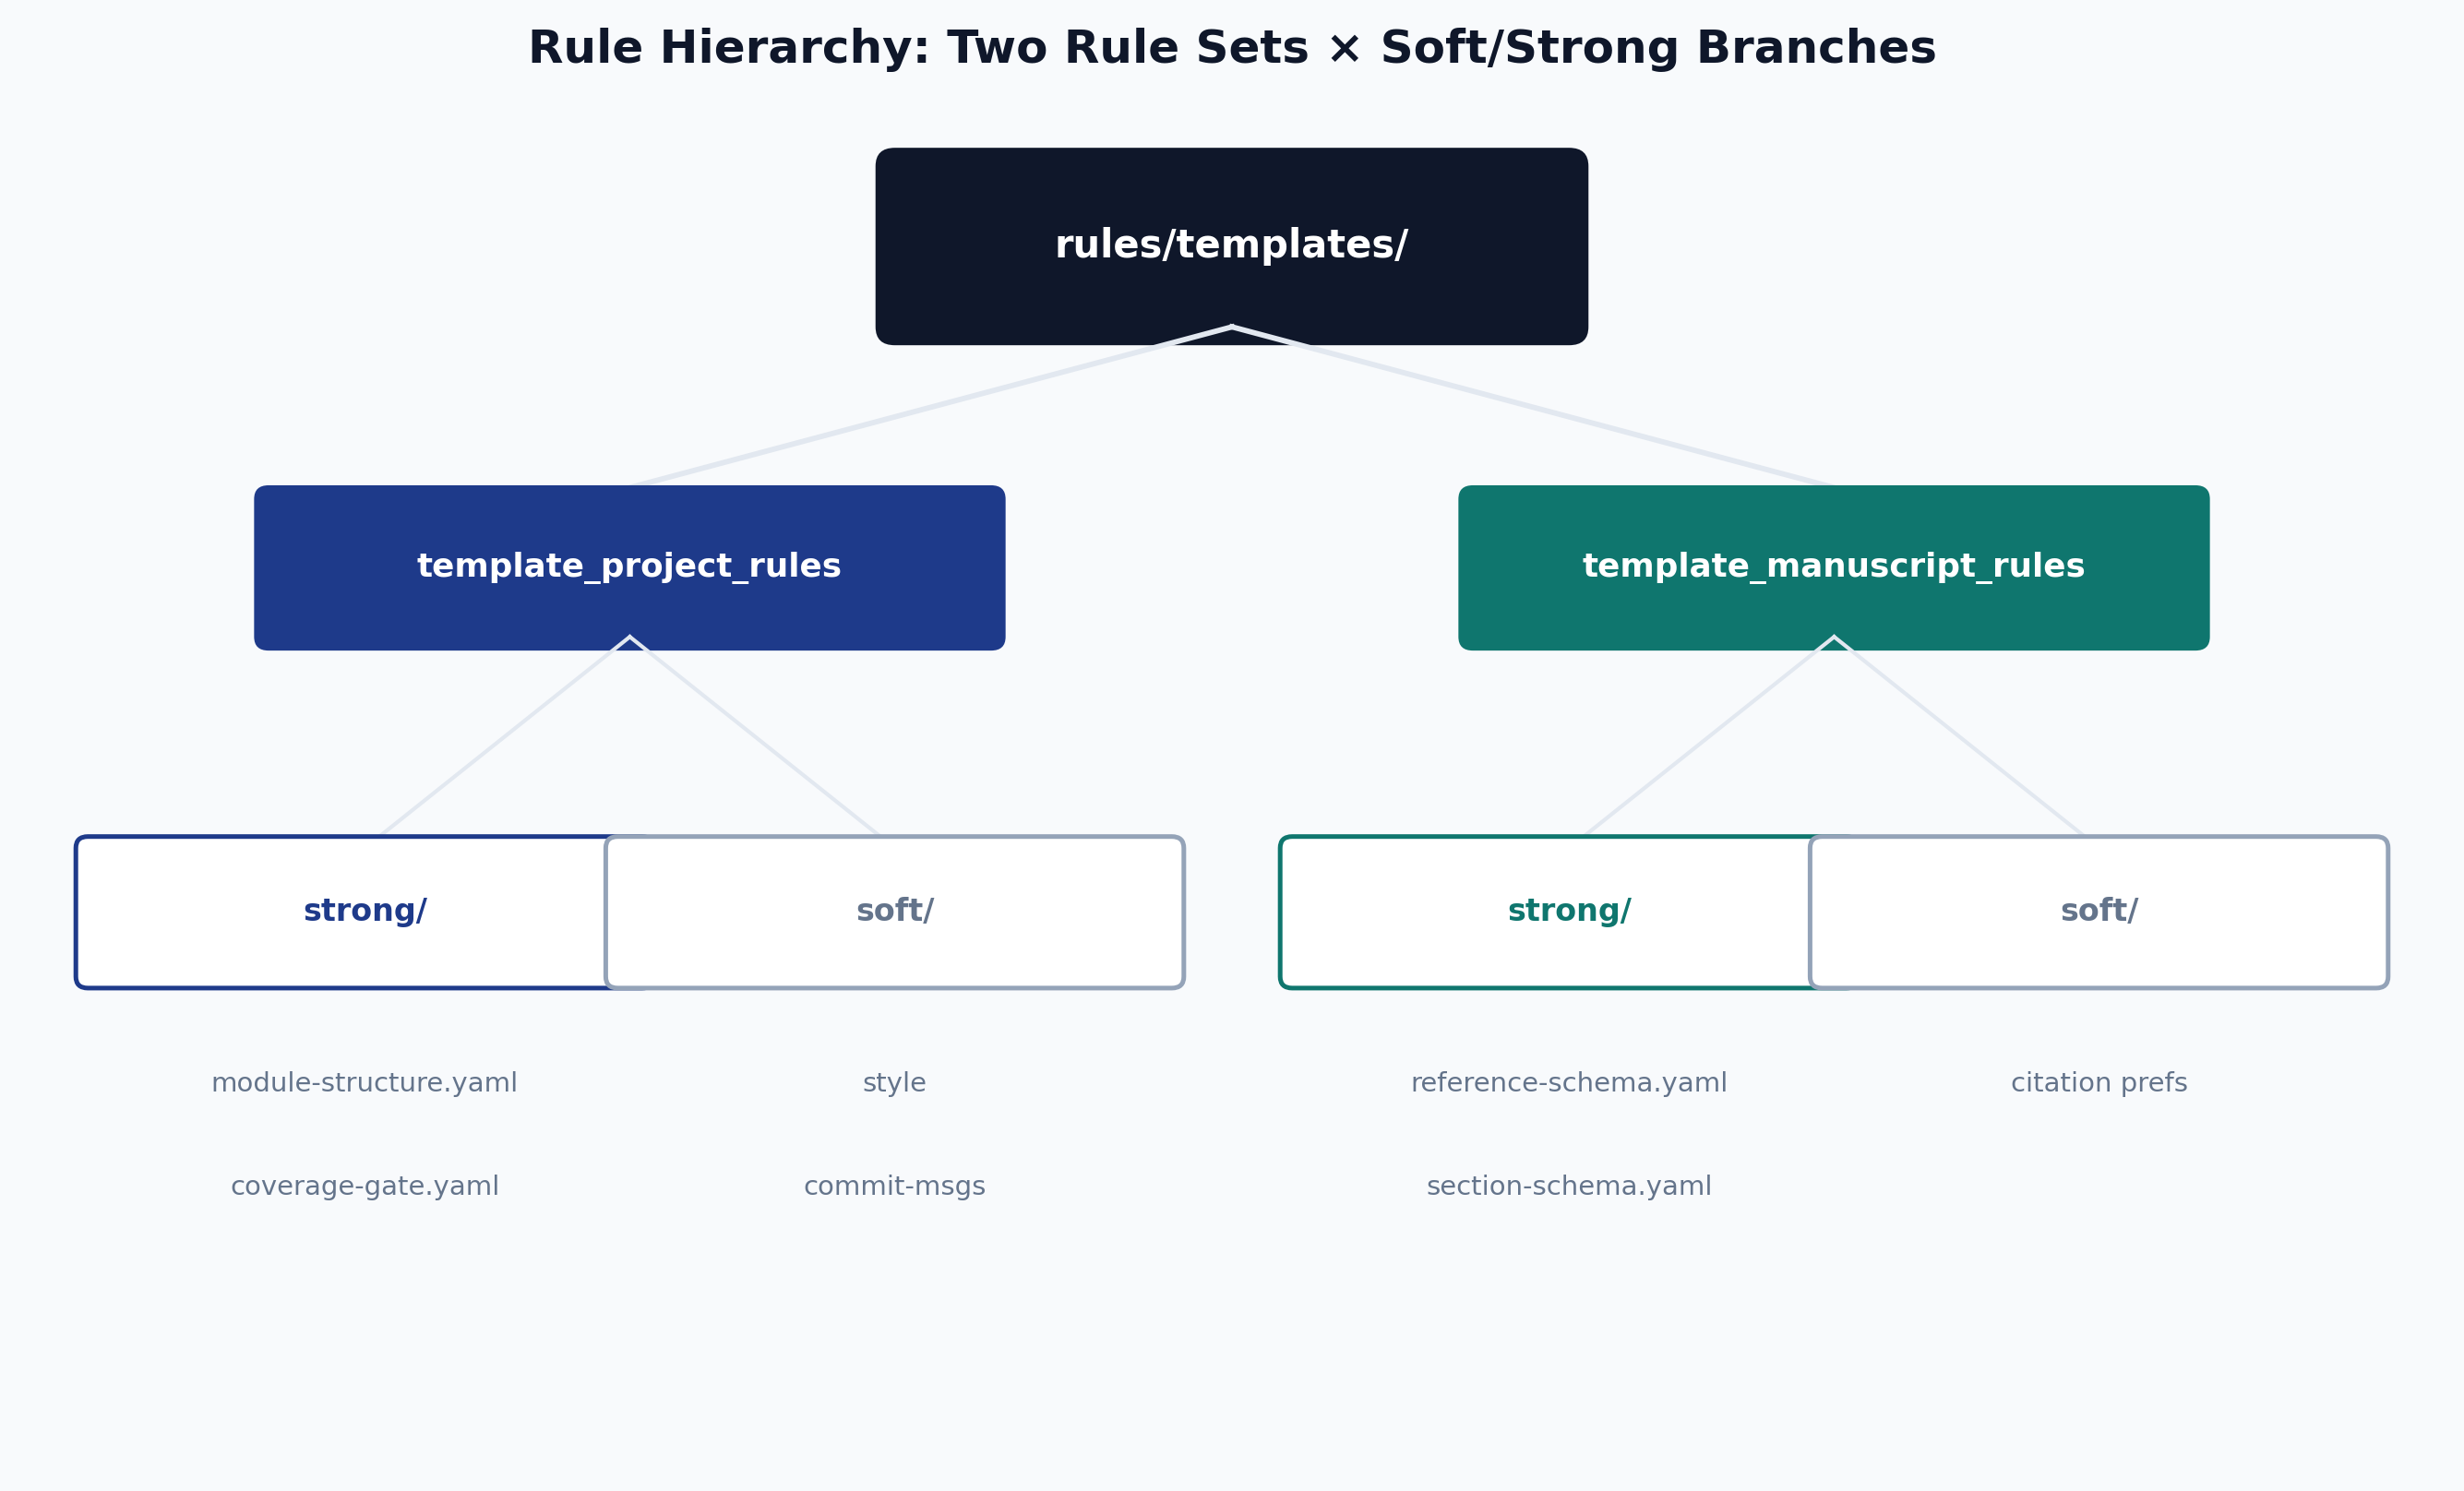
\includegraphics[width=0.85\linewidth,height=0.46\textheight,keepaspectratio,alt={Rule hierarchy: the two template rule sets, each split into a machine-enforceable strong/ branch and a guidance-only soft/ branch.}]{../figures/rule_hierarchy.png}
\caption{Rule hierarchy: the two template rule sets, each split into a
machine-enforceable \protect\texttt{strong/} branch and a guidance-only
\protect\texttt{soft/} branch.}\label{fig:rulehier}
\end{figure}
\end{frame}

\begin{frame}[fragile,allowframebreaks]{The Two Template Rule Sets}
\protect\phantomsection\label{the-two-template-rule-sets}
\begin{block}{\breaktt{template\_project\_rules}}
\protect\phantomsection\label{template_project_rules}
This rule set governs software projects throughout the template
repository. Its strong rules currently comprise:

{\def\LTcaptype{none} % do not increment counter
\begin{longtable}[]{@{}
  >{\raggedright\arraybackslash}p{(\linewidth - 2\tabcolsep) * \real{0.5000}}
  >{\raggedright\arraybackslash}p{(\linewidth - 2\tabcolsep) * \real{0.5000}}@{}}
\toprule\noalign{}
\begin{minipage}[b]{\linewidth}\raggedright
File
\end{minipage} & \begin{minipage}[b]{\linewidth}\raggedright
Constraint
\end{minipage} \\
\midrule\noalign{}
\endhead
\breaktt{strong/coverage-gate.yaml} & Minimum line coverage 90\%, branch
coverage 80\% for \texttt{src/} \\
\breaktt{strong/module-structure.yaml} & Required directory layout:
\texttt{src/}, \texttt{tests/}, \texttt{scripts/},
\texttt{manuscript/} \\
\bottomrule\noalign{}
\end{longtable}
}

Its soft rules provide guidance on code style, commit message
conventions, and pull-request labelling.
\end{block}

\begin{block}{\breaktt{template\_manuscript\_rules}}
\protect\phantomsection\label{template_manuscript_rules}
This rule set governs research manuscripts. Its strong rules comprise:

{\def\LTcaptype{none} % do not increment counter
\begin{longtable}[]{@{}
  >{\raggedright\arraybackslash}p{(\linewidth - 2\tabcolsep) * \real{0.5000}}
  >{\raggedright\arraybackslash}p{(\linewidth - 2\tabcolsep) * \real{0.5000}}@{}}
\toprule\noalign{}
\begin{minipage}[b]{\linewidth}\raggedright
File
\end{minipage} & \begin{minipage}[b]{\linewidth}\raggedright
Constraint
\end{minipage} \\
\midrule\noalign{}
\endhead
\breaktt{strong/reference-schema.yaml} & Required BibTeX fields and
cite-key format constraints \\
\breaktt{strong/section-schema.yaml} & Required manuscript sections,
ordering, and minimum word counts \\
\bottomrule\noalign{}
\end{longtable}
}

In the current pipeline run, \textbf{2 of 2 rule sets} validated
successfully (@fig:counts).
\end{block}
\end{frame}

\begin{frame}[fragile,allowframebreaks]{The \texttt{rules\_applier}
Module}
\protect\phantomsection\label{the-rules_applier-module}
The \breaktt{src/rules\_applier.py} module exposes three functions:

\begin{Shaded}
\begin{Highlighting}[]
\ImportTok{from}\NormalTok{ src.rules\_applier }\ImportTok{import}\NormalTok{ (}
\NormalTok{    load\_soft\_rules,}
\NormalTok{    load\_strong\_rules,}
\NormalTok{    validate\_against\_rules,}
\NormalTok{)}

\NormalTok{soft   }\OperatorTok{=}\NormalTok{ load\_soft\_rules(}\StringTok{"template\_project\_rules"}\NormalTok{)    }\CommentTok{\# list[dict]}
\NormalTok{strong }\OperatorTok{=}\NormalTok{ load\_strong\_rules(}\StringTok{"template\_project\_rules"}\NormalTok{)  }\CommentTok{\# list[dict]}
\NormalTok{result }\OperatorTok{=}\NormalTok{ validate\_against\_rules(}\StringTok{"template\_project\_rules"}\NormalTok{)}
\CommentTok{\# → \{"status": "ok" | "partial" | "missing", "soft\_count": N, "strong\_count": N\}}
\end{Highlighting}
\end{Shaded}

\breaktt{validate\_against\_rules()} performs two checks: (1) the
\texttt{rules.yaml} manifest is parseable YAML; (2) every rule file in
\texttt{soft/} and \texttt{strong/} is parseable YAML. It returns a
status of \texttt{"ok"} when both checks pass, \texttt{"partial"} when
the manifest exists but some rule files are missing or malformed, and
\texttt{"missing"} when the rule set directory is absent entirely. This
graduated status enables the integration pipeline to distinguish between
a rule set that has not yet been created (acceptable during active
development) and one that is present but broken (actionable defect).
\end{frame}

\begin{frame}[fragile,allowframebreaks]{Rules and Manuscript Variables}
\protect\phantomsection\label{rules-and-manuscript-variables}
Strong rule validation counts are injected into the manuscript through
the token system. The token \texttt{2} expands to the count of rule sets
that returned \texttt{status="ok"} during the integration run. This
creates a verifiable link between the pipeline's actual behaviour and
the manuscript's claims --- the manuscript cannot assert successful
validation without the pipeline having actually succeeded.
\end{frame}

\begin{frame}[fragile,allowframebreaks]{Beyond Structural Validation:
The \breaktt{strong\_rule\_evaluator} Module}
\protect\phantomsection\label{beyond-structural-validation-the-strong_rule_evaluator-module}
\breaktt{validate\_against\_rules()} (described above) performs
\emph{structural} validation only: it confirms that \texttt{rules.yaml}
and every file in \texttt{soft/}/\texttt{strong/} parse as YAML. It does
not check whether the constraints those strong-rule files declare are
actually satisfied by the current project. That semantic layer lives in
a separate module, \breaktt{src/strong\_rule\_evaluator.py}, exposed via
\breaktt{scripts/04\_validate\_strong\_rules.py}:

\begin{Shaded}
\begin{Highlighting}[]
\ImportTok{from}\NormalTok{ src.strong\_rule\_evaluator }\ImportTok{import}\NormalTok{ evaluate\_strong\_rules, load\_rule\_context\_from\_project}

\NormalTok{context }\OperatorTok{=}\NormalTok{ load\_rule\_context\_from\_project(project\_root)}
\NormalTok{result }\OperatorTok{=}\NormalTok{ evaluate\_strong\_rules(}\StringTok{"template\_project\_rules"}\NormalTok{, context)}
\CommentTok{\# → \{"rule\_set": ..., "evaluations": [...], "passed": bool, "violation\_count": int\}}
\end{Highlighting}
\end{Shaded}

\breaktt{evaluate\_strong\_rules()} dispatches each strong-rule YAML file
to a rule-kind-specific evaluator function keyed by its declared kind,
via a small dispatch table covering all four strong-rule kinds that
exist across both rule sets:

{\def\LTcaptype{none} % do not increment counter
\begin{longtable}[]{@{}
  >{\raggedright\arraybackslash}p{(\linewidth - 4\tabcolsep) * \real{0.3333}}
  >{\raggedright\arraybackslash}p{(\linewidth - 4\tabcolsep) * \real{0.3333}}
  >{\raggedright\arraybackslash}p{(\linewidth - 4\tabcolsep) * \real{0.3333}}@{}}
\toprule\noalign{}
\begin{minipage}[b]{\linewidth}\raggedright
Kind
\end{minipage} & \begin{minipage}[b]{\linewidth}\raggedright
Evaluator
\end{minipage} & \begin{minipage}[b]{\linewidth}\raggedright
Checks
\end{minipage} \\
\midrule\noalign{}
\endhead
\breaktt{coverage\_threshold} & \breaktt{\_evaluate\_coverage\_threshold}
& Measured coverage percentages (from \texttt{context{[}"coverage"{]}})
against each constraint's declared \breaktt{minimum\_line\_coverage} \\
\breaktt{module\_structure} & \breaktt{\_evaluate\_module\_structure} &
Required project directory layout (\texttt{src/}, \texttt{tests/},
\texttt{scripts/}, \texttt{manuscript/}) actually exists \\
\texttt{section\_schema} & \breaktt{\_evaluate\_section\_schema} &
Required manuscript sections, ordering, and forbidden placeholder
headings (\texttt{TODO}, \texttt{Draft}, etc.) \\
\breaktt{reference\_schema} & \breaktt{\_evaluate\_reference\_schema} &
Required BibTeX fields and cite-key format constraints on every parsed
reference entry \\
\bottomrule\noalign{}
\end{longtable}
}

Each evaluator distinguishes structured violation \emph{reasons} rather
than collapsing everything to a boolean --- for example,
\breaktt{coverage\_threshold} reports separately whether a key was absent
from context (a context-completeness issue), non-numeric (a
context-shape issue), or numeric-but-below-minimum (a genuine rule
violation). This is what lets the pipeline tell a maintainer \emph{why}
a rule failed, not merely \emph{that} it failed --- directly addressing
the ``actionable defect'' distinction introduced in the previous
section.

Crucially, \texttt{section\_schema} and \breaktt{reference\_schema} are
not evaluated against synthetic fixtures ---
\breaktt{load\_rule\_context\_from\_project()} (in
\breaktt{scripts/04\_validate\_strong\_rules.py}) builds their context by
parsing \emph{this project's own, current}
\breaktt{manuscript/references.bib} into structured reference entries and
extracting the real \texttt{\#}-level headings from every file under
\texttt{manuscript/*.md}. Running
\breaktt{uv\ run\ python\ projects/templates/template\_pools\_rules\_tools/scripts/04\_validate\_strong\_rules.py}
therefore semantically validates this exact manuscript's own
bibliography and section structure, live, on every invocation --- re-run
that command to see the current evaluation and violation counts rather
than trusting a number printed here, since either count can legitimately
change as the manuscript grows.
\end{frame}

\end{document}
